% use paper, or submit
% use 11 pt (preferred), 12 pt, or 10 pt only

\documentclass[letterpaper, preprint, paper,11pt]{AAS}	% for preprint proceedings
%\documentclass[letterpaper, paper,11pt]{AAS}		% for final proceedings (20-page limit)
%\documentclass[letterpaper, paper,12pt]{AAS}		% for final proceedings (20-page limit)
%\documentclass[letterpaper, paper,10pt]{AAS}		% for final proceedings (20-page limit)
%\documentclass[letterpaper, submit]{AAS}			% to submit to JAS

\usepackage{AAS_packages}
%\usepackage{subfigure} % have subcaption in use instead
%\usepackage[notref,notcite]{showkeys}  % use this to temporarily show labels

% Macros for discrete states to save some time typing
\newcommand{\xk}{\ensuremath{x_k}}
\newcommand{\xkp}{\ensuremath{x_{k+1}}}
\newcommand{\yk}{\ensuremath{y_{k}}}
\newcommand{\ykp}{\ensuremath{y_{k+1}}}

\newcommand{\pxk}{\ensuremath{p_{x_k}}}
\newcommand{\pxkp}{\ensuremath{p_{x_{k+1}}}}
\newcommand{\pyk}{\ensuremath{p_{y_k}}}
\newcommand{\pykp}{\ensuremath{p_{y_{k+1}}}}

\newcommand{\distonek}{\ensuremath{r_{1_k}}}
\newcommand{\distonekp}{\ensuremath{r_{1_{k+1}}}}
\newcommand{\disttwok}{\ensuremath{r_{2_{k}}}}
\newcommand{\disttwokp}{\ensuremath{r_{2_{k+1}}}}

\PaperNumber{XX-XXX}



\begin{document}

\title{Systematic Design of Optimal Low-Thrust Transfers for the Three-Body Problem}

\author{Shankar Kulumani\thanks{Doctoral Student, Mechanical and Aerospace Engineering, George Washington University, 801 22nd St NW, Washington, DC 20052, Email: \href{mailto:skulumani@gwu.edu}{skulumani@gwu.edu}.},  
Taeyoung Lee\thanks{Associate Professor, Mechanical and Aerospace Engineering, George Washington University, 801 22nd St NW, Washington, DC 20052, Tel: 202-994-8710, Email: \href{mailto:tylee@gwu.edu}{tylee@gwu.edu}.}
}


\maketitle{} 		


\begin{abstract}
Concise summary

general topic is mentioned first

how it relates to previous work

new developments in paper

summary of the contents of this paper

\end{abstract}


\section{Introduction}\label{sec:introduction}
% MOTIVATION FOR LOW THRUST ORBITAL TRANSFER 
Designing spacecraft trajectories is a classic and ongoing topic of research.
With the current fiscal constraints there is an increased focused on technologies with a critical impact on mass.
Optimal expenditure of onboard propellant is critical to allowing a mission to continue for a longer period of time or to enable the launch of a less massive spacecraft.
Electric propulsion systems offer a much greater specific impulse than chemical systems and are able to operate for extended periods of time.
However, these electric propulsion systems typically have much less thrust than their chemical counterparts and therefore must operate over longer durations in order to impart the desired momentum change.
Recent developments in miniature electric propulsion~\cite{haque2013} offer the potential for new research opportunities for small spacecraft.
With reduced development intervals and decreased launch costs, small satellites have gained increased focus as a cost effective means of scientific and technologic development. 
The merger of small satellites with miniature electric propulsion enables inexpensive and responsive missions requiring large changes in orbital energy or extended mission lifespan.
With the potential for more demanding missions, even greater importance is placed on the mission design to ensure that optimal trajectories satisfy mission requirements. 
In addition, non-Keplerian orbits and multi-body dynamics have been shown to allow for a much greater range of potential missions at a reduced energy cost~\cite{koon2000}.
Future space missions are increasing in complexity and will require new classes of orbits that are not possible via the traditional conic approach~\cite{ross2006,gomez2001}.
Optimally combining the dynamical structure of the three-body problem with low-thrust propulsion system is vital for future mission success.

% PRIOR WORK AND CHALLENGES
Much work has focused on optimal control for spacecraft orbital transfers in the three-body problem~\cite{mingotti2011,grebow2011}.
Typically, the optimal control problem is solved via direct methods, which approximate the continuous problem as a parameter optimization problem.
The state and/or control trajectories are parameterized and solved in the form of a nonlinear optimization problem.
References~\citenum{mingotti2011} and~\citenum{grebow2011} use this direct approach in designing low-thrust transfers in the three-body problem.
Alternatively, indirect methods apply calculus of variations to derive the necessary conditions for optimality. 
This yields a lower dimensioned problem than the direct approach and algebraic conditions that, when satisfied, guarantee local optimality in contrast to direct methods which result in sub-optimal solutions.

Additionally, References~\citenum{mingotti2011} and~\citenum{grebow2011} implement the solutions using conventional Runge-Kutta integration techniques.
These techniques suffer from numerical instability and energy drift behaviors which make them ill-suited for long-term propagation.
These dissipative effects are even more detrimental with the addition of low-thrust propulsion to the dynamic equations of motion.
Conventional integration techniques fail to capture the physical laws and geometric properties of the dynamic system.
As a result, the long term effects of low-thrust on the spacecraft trajectory are not accurately captured. 

References~\citenum{koon2000} and~\citenum{ross2006} have illustrated the rich structure that exists in the three-body problem.
Within the three-body problem, a spacecraft's feasible region of motion is constrained by it's energy, or Jacobi integral. 
It has been shown that there exist multi-dimensional tubes, or invariant manifolds, of constant energy trajectories that span the state space. 
Associated with periodic solutions of the three-body dynamics, these invariant manifolds allow for the spacecraft to traverse vast expanses of the state space with zero energy change. 
However, the results presented are highly case specific and difficult to generalize to arbitrary transfers.
Also, these results are based on control-free trajectories which rely on the underlying structure of the three-body system.
In addition, transfer orbits along an invariant manifold require large time of flights which may be undesirable for time critical missions.
The addition of low-thrust propulsion offers the potential of reduced transit times and the ability to depart from the free motion trajectory to allow for increased transfer opportunities. 

% OBJECTIVE OF THIS WORK
In order to address these issues the authors propose to develop a accurate and numerically stable method for long-term optimal orbital transfers.
This approach will avoid the instability and dissipative effects of conventional integration schemes.
In addition, the effects of low-thrust propulsion will be directly included in the integration method to ensure that extended duration optimal trajectories are computed correctly.
This improved method will enable the derivation of a systematic method of generating optimal transfer orbits between arbitrary states.
Indirect optimal control, based on the calculus of variations, will be implemented in order to generate optimal orbital transfers.
This will avoid the approximation issues inherent in the previous work, which utilized direct optimal control methods.
With this proposed method, the previous research on control-free trajectories will be generalized with the addition of low-thrust propulsion systems.

% TECHNICAL DESCRIPTION OF APPROACH
To achieve these objectives, computational geometric optimal control techniques will be applied. 
The dynamics of the three-body system are derived from the discrete Lagrangian, which approximates the integral of the continuous time Lagrangian over a fixed discrete step.
Application of the discrete Euler-Lagrange equations, or the discrete Legendre transform, results in the discrete equations of motion.
This discrete update map, or variational integrator, shares the same geometric properties of the continuous time system and exhibits much better energy behavior than the traditional integration methods, especially over long time periods.
A discrete optimal control problem is formulated from the discrete equations of motion.
This approach, where explicit discretization occurs prior to optimization,  is in contrast to the typical method, where the equations of motion are implicitly discretized during the optimization procedure.
Formulating the problem in this manner results in a more stable and accurate optimal solutions. 
In indirect methods the optimal control problem is expressed as a two-point boundary value problem.
Optimal solutions are generally sensitive to small variations in the initial multipliers.
As a result, the numerical stability of sensitivity derivatives is critical to accuracy and computational performance. 
The use of geometric integrators, which do not suffer the numerical dissipation of conventional integration methods, results in a more robust and efficient solution.

A discrete optimal control problem is formulated to determine the reachability set on a Poincar\'e section.
Given an initial condition and fixed time horizon, the reachable set is the set of states attainable, subject to the operational constraints of the spacecraft. 
Generation of this reachability set allows for the extension of the previous control-free missions in the three-body problem. 
The addition of low-thrust propulsion affords the ability to enlarge the reachable set as compared to the control-free case.
Maximization of the reachability set, on an appropriately chosen Poincar\'e section, allows for a greater space of potential transfer trajectories.
The use of the Poincar\`e section allows for design on a lower dimensional space and simplifies the design process.
Once an intersection is determined on the Poincar\`e section a transfer is calculated.

% SUMMARY OF CONTRIBUTIONS
In this paper, the authors develop a systematic method of generating optimal transfer orbits in the three-body problem.
Previous results in the design of optimal transfers have relied on suboptimal direct optimization methods and conventional integration techniques.
This paper provides a discrete optimal control formulation to generate the reachability set on a Poincar\'e section.
The use of a geometric integrators ensures numerical stability for long-duration orbit transfers.

\section{System Model}\label{sec:pcrtbp}
The system model is based on the planar circular restricted three body problem~(PCRTBP).
The Earth is assumed to be the more massive primary, \( m_1 \), while the Moon is the second, smaller primary \( m_2\).
The equations of motion are developed in a rotating reference frame which allows for much greater insight into the structure of the dynamics.
The \( \hat{x} \) axis is directed along the vector from the Earth to the Moon.
The \( \hat{y} \) axis lies in the orbital plane and is orthogonal to \( \hat{x} \).
The rotating reference frame is centered at the system barycenter.
It is assumed that the the \(\left( \hat{x}, \hat{y}\right)\) rotates with a constant angular velocity equal to the mean motion of the Moon.
Following convention, the system is also non-dimensionalized by the characteristic mass, length, and time~\cite{koon2000}.
As a result, the system can be characterized by a single mass parameter \( \mu \).
\begin{equation}
	\mu = \frac{m_2}{m_1+m_2}
	\label{eq:mass_param}
\end{equation}
The larger primary, \(m_1\), is located at \( \left(  -\mu , 0 \right)\) and the smaller \( m_2\) is located at \( \left( 1-\mu , 0 \right)\).
In the rotating reference frame the Lagrangian is given by
\begin{equation}
	L = \frac{1}{2} \left( \left( \dot{x} -y \right)^2 + \left( \dot{y} + x \right)^2 \right) + \frac{1-\mu}{r_1} + \frac{\mu}{r_2}
	\label{eq:lagrangian}
\end{equation}
where the distance \(r_1\) and \(r_2\) of the spacecraft to each primary is defined in rotating coordinates as
\begin{align}
	r_1 &= \sqrt{\left( x + \mu\right)^2 + y^2} \\
	r_2 &= \sqrt{\left( x - 1 + \mu\right)^2 + y^2}
	\label{eq:distances}
\end{align}
Application of the Euler-Lagrange equations results in following equations of motion defined in the rotating reference frame
\begin{align}
	\ddot{x} - 2 \dot{y} + \frac{\partial}{\partial x} U &= u_x \nonumber \\
	\ddot{y} + 2 \dot{y} + \frac{\partial}{\partial y} U &= u_y 
	\label{eq:cont_eom}
\end{align}
where the effective potential \( U\) is defined as
\begin{equation}
	U = \frac{1}{2} \left( x^2 y^2\right) + \frac{1-\mu}{r_1} + \frac{\mu}{r_2}
	\label{eq:eff_pot}
\end{equation}
and the control inputs are defined as \( u_x\) and \(u_y\).
Defining the state \( \bar{x} = \begin{bmatrix}\bar{r} &\bar{v} \end{bmatrix}\) with \(\bar{r} \in \R^{2\times1}\) and \(\bar{v} \in \R^{2\times1}\) representing the position and velocity with respect to the system barycenter, respectively.
The equations of motion may be rewritten in state space form
\begin{equation}
	\left[\begin{array}{c} \dot{\bar{r}} \\ \dot{\bar{v}} \end{array} \right] = 
	\left[ \begin{array}{c} \bar{v} \\ A \bar{v} + \nabla U + \bar{u}(t) \end{array} \right] = f\left( t,x, u\right)
\end{equation}
where the matrix \( A \) and psuedo gravitational potential gradient \( \nabla U\) are
\begin{equation}\label{eq:A_mat}
	A = \left[ \begin{array}{ccc} 0 & 2 & 0 \\ -2 & 0 & 0 \\ 0 & 0 & 0 \end{array} \right]
\end{equation}
\begin{equation} \label{eq:grav_pot}
	\nabla U = \left[ \begin{array}{c} x - \frac{ \left(1 - \mu\right) \left(x + \mu\right)}{r_1^3} - \frac{\mu \left( x+ \mu -1\right)}{r_2^3} \\
											y - \frac{ \left(1 - \mu\right) y}{r_1^3} - \frac{\mu y}{r_2^3} \\
											- \frac{ \left(1 - \mu\right) z}{r_1^3} - \frac{\mu z}{r_2^3}\end{array}\right]
					= \left[\begin{array}{c} U_x \\ U_y \\ U_z\end{array} \right]
\end{equation}

\subsection{Jacobi Integral}
There exists a single integral, or constant of motion for the three-body problem~\cite{lanczos1970,szebehely1967}.
This energy constant is analogous to the total mechanical energy, however is a non physical quantity arising from the problem formulation~\cite{szebehely1967}.
Also known as the Jacobi constant, it is defined as a function of the position and velocity in the rotating frame
\begin{equation}
	E\left( \bar{r} , \bar{v} \right) = \frac{1}{2}\left( \dot{x}^2 + \dot{y}^2\right) - U\left(x,y \right)
	\label{eq:jacobi}
\end{equation}
The Jacobi integral~\eqref{eq:jacobi} divides the phase space into distinct regions based on the energy level of the body of interest.
Fixing the Jacobi integral to a constant defines zero velocity curves, which are the locus of points where the kinetic energy, and hence velocity vanishes.
As seen in Figure~\ref{fig:energy_contour}, the phase space is divided into distinct realms based on the energy level.
\begin{figure}[htbp]
	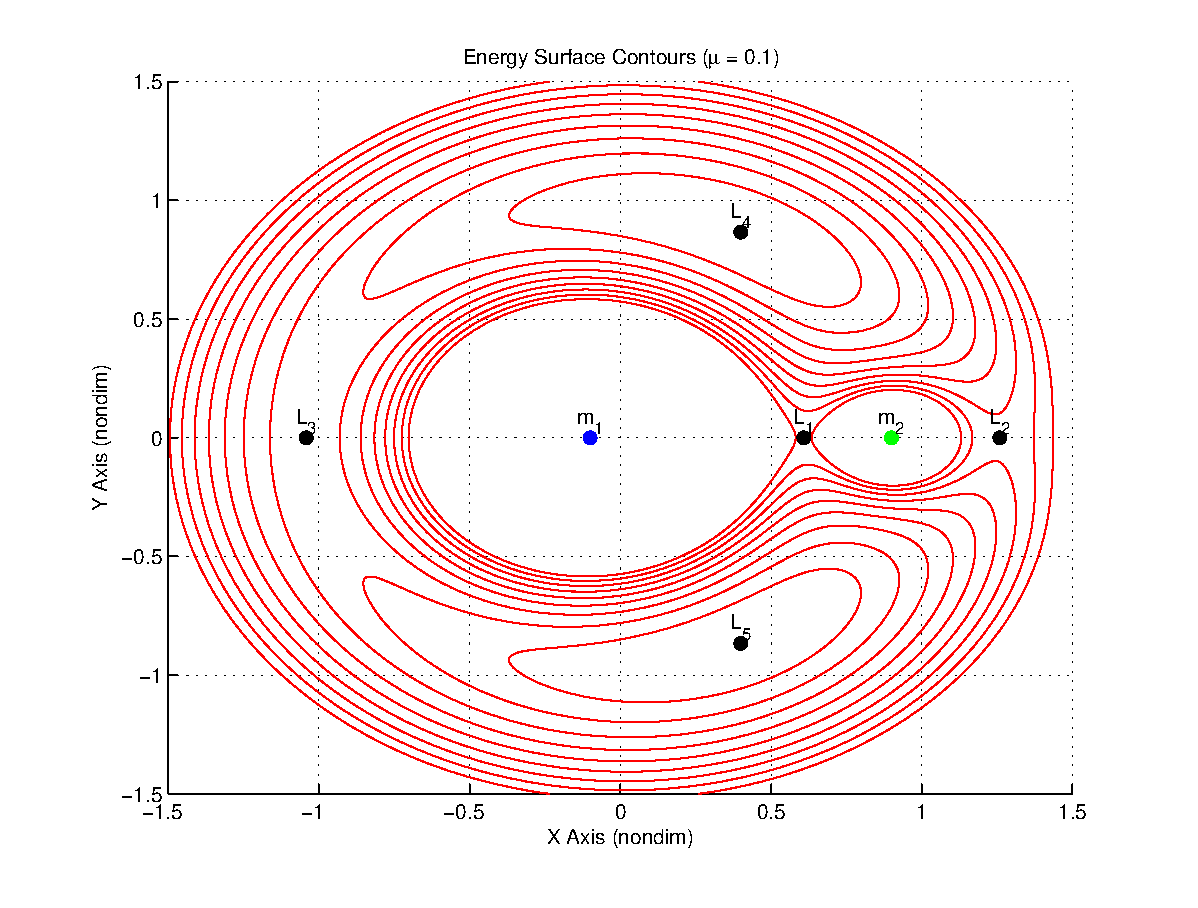
\includegraphics[width=\textwidth]{energy_contours}
	\caption{Contour Plot of Jacobi Integral}
	\label{fig:energy_contour}
\end{figure} 
In the vicinity of \( m_1\) or \(m_2\) we have a potential well. 
As the energy level increases we find that there are five critical points of the effective potential~\eqref{eq:eff_pot} where the slope is zero.
Three collinear saddle points on the \(x\) axis and two symmetric points off the \(x\) axis.
These equilibrium, or Lagrange points, are labeled \( L_i, i = 1, \hdots, 5 \) and are shown in Figure~\ref{fig:energy_contour}.

\subsection{Periodic Orbits and Invariant Manifolds}
Used to generate a Periodic orbit about a lagrange point
Periodic orbits about the lagrange points
\subsection{Poincar\`e Section}
Intersection of states with a lower dimensional plane
Introduce invariant manifolds

\section{Geometric Variational Integrator}\label{sec:discrete_var}
% description of variational integrator development
Geometric numerical integration deals with numerical integration methods which preserve the geometric properties of the flow of a differential equation, such as invaraint properties and symplecticity.
Variational integrators are constructed by discretizing Hamilton's principle rather than the continuous Euler-Lagrange equations~\cite{marsden2001}.
As a result, integrators developed in this manner have the desirable properties that they are symplectic and momentum preserving.
In addition, they exhibit improved energy behavior over long integration periods.
A short background on the variational principle for mechanical systems is presented. 
A discrete approximation of the action integral is presented and allows for construction of a variational integrator for the PCRTBP.

\subsection{Variational Principle}
Consider a continuous mechanical system described by the Lagrangian, \( L( q, \dot{q} ) \), for the generalized position and velocity \( q, \dot{q} \), respectively.
In the standard approach of variational mechanics we form the action integral by integrating the continuous Lagrangian along a path \( q(t) \) that the system follows from time \( t = 0 \) to \( t = T \)~\cite{greenwood1988}.
In the continuous time the action integral is defined as
\begin{align}\label{eq:action_integral}
	S = \int_{0}^T L\left( q, \dot{q}\right) \, dt
\end{align}
Hamilton's principle states that the actual path followed by a holonomic system results in a stationary action integral with respect to path variations for fixed endpoints.
Taking the variation of~\cref{eq:action_integral} gives
\begin{subequations}
\begin{align}\label{eq:var_principle}
	\delta S &= \int_{0}^T \deriv{L}{q} \delta q + \deriv{L}{\dot{q}} \delta \dot{q} \, dt \\
		&= \int_{0}^T \deriv{L}{q} \delta q - \frac{d}{dt} \left( \deriv{L}{\dot{q}}\right) \delta q \, dt - \left. \left[ \deriv{L}{\dot{q}} \delta q\right] \right|_0^T \\
	&= \int_{0}^T \deriv{L}{q} - \frac{d}{dt} \left( \deriv{L}{\dot{q}}	\right)
\end{align}
\end{subequations} 
where we have used integration by parts and the conditions \( \delta q(0) = 0 \) and \( \delta q(T) = 0\).
For Hamilton's principle to be valid for all admissible variations \( \delta q \), the integrand of~\cref{eq:var_principle} must be zero for all \( t\), giving the continuous Euler-Lagrange Equations~\cite{lanczos1970}.
\begin{align}\label{eq:euler-lagrange}
	0 = \deriv{L}{q} - \frac{d}{dt} \left( \deriv{L}{\dot{q}} \right) 
\end{align}
Hamilton's equations are derivable through the use of the Legendre transformation which is a mapping \( \left( q, \dot{q},t\right) \rightarrow \left(q, p, t \right) \) where \( p_i\) is the generalized momenta.
\begin{align}\label{eq:legendre_transform}
	p_i = \deriv{L}{\dot{q}}
\end{align}
In the continuous time case one can define the Hamiltonian
\begin{align}\label{eq:hamiltonian}
	H &= \sum_{i = 1}^N p_i \dot{q}_i - L \left( q_i,\dot{q}_i, t \right)
\end{align}
Applying~\cref{eq:legendre_transform} and taking the variation of~\cref{eq:hamiltonian} allows us to derive the equations of motion in Hamiltonian form
\begin{subequations}
\begin{align}\label{eq:hamilton_eq}
	\dot{q}_i &= \deriv{H}{p_i} \\
	\dot{p}_i &= - \deriv{H}{q_i} + Q_i \\
	\deriv{L}{t} &= -\deriv{H}{t}
\end{align}
\end{subequations}
Both~\cref{eq:euler-lagrange,eq:hamilton_eq} result in equations of motion for the mechanical system and are equivalent via the Legendre transform.
\Cref{eq:euler-lagrange} results in \( n \) second order differential equations while~\cref{eq:hamilton_eq} results in \( 2n \) first order differential equations.
\subsection{Discrete Variational Mechanics}
A discrete analogue of Hamilton's principle and the action integral is formed.
Rather than taking a position \( q \) and velocity \( \dot{q} \), consider two positions \( q_0 \) and \( q_1 \) and a fixed time step \( h \in \R \).
The two positions are points on the curve \( q(t) \) such that \( q_0 \approx q(0) \) and \( q_1 \approx q(h) \).
A discrete time Lagrangian \( L_d( q_0, q_1) \) is formed which approximates the action integral between \( q_0 \) and \( q_1 \). 
\begin{align}\label{eq:discrete_lagrangian}
	L_d\left( q_0 , q_1 \right) \approx \int_{0}^{h} L \left( q , \dot{q} \right) \, dt
\end{align}
Since~\cref{eq:discrete_lagrangian} is calculated as a numerical integral an appropriate quadrature rule is required.
There are multiple possible methods one can use to approximate the integral in~\cref{eq:discrete_lagrangian}.
An appropriate approximation rule is determined based on the ease of implementation and accuracy desired.
\begin{table}[htbp]
\begin{center}\begin{tabular}{l|l}Rectangle & \( L_d(q_0,q_1) =L(q_0,\frac{q_1-q_0}{h}) h \)  \\ \hline
Midpoint & \( L_d(q_0,q_1) = L(\frac{q_0 + q_1}{2},\frac{q_1 - q_0}{h}) h \) \\ \hline
Trapezoidal & \( L_d(q_0, q_1) = \frac{1}{2} \left[ L(q_0, \frac{q_1 - q_0}{h} ) + L(q_1, \frac{q_1 - q_0 }{h} )\right] h \)
\end{tabular} 
\caption{Selected Quadrature Rules}
\end{center}
\label{tab:quadrature}
\end{table}
The rectangle rule is a first order accurate method and offers a straightforward implementation.
The midpoint and trapezoidal rules are both second order accurate methods. 
However, the midpoint rule results in an implicit form which adds further complexity to the equations of motion.
In this work, the trapezoidal approximation is applied to the PCRTBP.

Once an appropriate discrete Lagrangian is formed a discrete action sum is formed as the discrete analogue of~\cref{eq:action_integral}
\begin{align}\label{eq:action_sum}
	S_d = \sum_{k=0}^{N-1} L_d(q_k, q_{k+1})
\end{align}
Once again, a discrete version of Hamilton's principle is applied to~\cref{eq:action_sum}, and applying summation by parts yields
\begin{subequations}
\begin{align}\label{eq:dis_var_principle}
	\delta S_d &= \sum_{k=0}^{N-1} \deriv{L_d(q_k, q_{k+1}}{q_k} \delta q_k + \deriv{L_d(q_k, q_{k+1})}{q_{k+1}} \delta q_{k+1} \\
	&= \sum_{k=1}^{N-1} \bracket{ \deriv{L_d(q_k, q_{k+1}}{q_k} + \deriv{L_d(q_{k-1}, q_k)}{q_{k+1}}} \delta q_k
\end{align}
\end{subequations}
For the discrete action sum to be stationary with respect to all admissible path variations, with fixed endpoints, the discrete Euler-Lagrange equations must be satisfied for \( k = 1, \cdots, N-1 \).
\begin{align}\label{eq:discrete_euler-lagrange}
	0 = \deriv{L_d(q_k, q_{k+1}}{q_k} + \deriv{L_d(q_{k-1}, q_k)}{q_{k+1}}
\end{align}
Similarly, a discrete version of the Legendre transformation, referred to as a discrete fiber derivative the equivalent Hamiltonian form expression is
\begin{subequations}\label{eq:discrete_legendre}
\begin{align}
	p_k &= \deriv{L_d(q_{k-1},q_k)}{q_{k+1}} = - \deriv{L_d(q_k, q_{k+1})}{q_k} \\
	p_{k+1} &= \deriv{L_d(q_k, q_{k+1})}{q_{k+1}}
\end{align}
\end{subequations}
This yields a discrete Hamiltonian map \( (q_k, p_k) \to (q_{k+1}, p_{k+1}) \).
A more extensive development of variational integrators can be found in Reference~\citenum{marsden2001}.

\subsection{Discrete Equations of Motion}
The discrete equations of motion for the PCRTBP are derived by choosing an appropriate quadrature rule to discretize the Lagrangian in~\cref{eq:lagrangian}. 
In this work, the trapezoidal approximation is applied.
The trapezoid rule allows for an explicit second order accurate approximation.
The discrete Lagrangian is given by
\begin{align}\label{eq:discrete_lagrangian}
	L_d &= \frac{h}{2} \left( \frac{1}{2} \bracket{\left(  \frac{\xkp - \xk}{h} -\yk \right)^2 + \left( \frac{\ykp - \yk}{h} + \xk \right)^2} + \frac{1 - \mu}{r_{1_k}} + \frac{\mu}{r_{2_k}} \right. \nonumber \\ 
	&+ \left. \frac{1}{2} \bracket{\left(  \frac{\xkp - \xk}{h} -\ykp \right)^2 + \left( \frac{\ykp - \yk}{h} + \xkp \right)^2} + \frac{1-\mu}{r_{1_{k+1}}} + \frac{\mu}{r_{2_{k+1}}}  \right)
\end{align}
Applying a discrete version of the Lagrange-d?Alembert principle allows for inclusion of an external control force on the system~\cite{marsden2001}.
Using~\cref{eq:discrete_legendre,eq:discrete_lagrangian} and some manipulation the equations of motion are given by
\begin{subequations}\label{eq:discrete_eoms}
\begin{align}
	\xkp &= \frac{1}{1+ h^2} \bracket{h \dot{x}_k - h \yk + h^2 \dot{y}_k + h^2 \xk + \xk \parenth{1+ \frac{h^2}{2}} + \yk \parenth{h + \frac{h^3}{2}} - \frac{h^3}{2} U_{y_k} - \frac{h^2}{2} U_{x_k} } \label{eq:xkp}\\
	\ykp &= h \dot{y}_k + h \xk - h \xkp + \yk + \frac{h^2 \yk}{2} - \frac{h^2 }{2} U_{y_k} \label{eq:ykp}\\
	\dot{x}_{k+1} &= \dot{x}_k - 2 \yk + 2 \ykp + \frac{h}{2} \parenth{\xkp + \xk} - \frac{h}{2} U_{\xkp} - \frac{h}{2} U_{\xk} + h u_x \label{eq:xdotkp}\\
	\dot{y}_{k+1} &= \dot{y}_{k+1} + 2 \xk - 2 \xkp + \frac{h}{2} \parenth{\ykp + \yk} - \frac{h}{2} U_{\ykp} - \frac{h}{2} U_{\yk} + h u_y \label{eq:ydotkp}
\end{align}
\end{subequations}
The discrete equations of motion are given in the Lagrangian form after applying the discrete Legendre transform from~\cref{eq:discrete_legendre} as \( p_{\xk} = \dot{x}_k - \yk \) and \( p_{\yk} = \dot{y}_k + \xk \).
The state is defined as \( \bar{ x}_k = \begin{bmatrix} \xk & \yk & \dot{x}_k & \dot{y}_k \end{bmatrix}^T\) and the control input is \( \bar{u} = \begin{bmatrix} u_x & u_y \end{bmatrix}^T \).
The discrete potential gradients are given by
\begin{subequations}\label{eq:discrete_potential_grad}
\begin{align}
	U_{\xk} &= \frac{\parenth{1 -\mu} \parenth{\xk + \mu}}{\distonek^3} + \frac{ \mu \parenth{\xk -1 + \mu}}{\disttwok^3} \label{eq:Uxk}\\
	U_{\yk} &= \frac{\parenth{1 -\mu} \yk}{\disttwok^3} + \frac{ \mu \yk}{\disttwok^3} \label{eq:Uyk} \\
	U_{\xkp} &= \frac{\parenth{1 -\mu} \parenth{\xkp + \mu}}{\distonekp^3} + \frac{ \mu \parenth{\xkp -1 + \mu}}{\disttwokp^3} \label{eq:Uxkp}\\
	U_{\ykp} &= \frac{\parenth{1 -\mu} \ykp}{\distonekp^3} + \frac{ \mu \ykp}{\disttwokp^3} \label{eq:Uykp}
\end{align}	
\end{subequations}
The distances to each primary are defined as
\begin{subequations}\label{eq:discrete_distance}
\begin{align}
	\distonek &= \sqrt{\left( \xk + \mu\right)^2 + \yk^2} \label{eq:distonek}\\
	\disttwok &= \sqrt{\left( \xk - 1 + \mu\right)^2 + \yk^2} \label{eq:disttwok}\\
	\distonekp &= \sqrt{\left( \xkp - 1 + \mu\right)^2 + \ykp^2} \label{eq:distonekp}\\
	\disttwokp &= \sqrt{\left( \xkp - 1 + \mu\right)^2 + \ykp^2} \label{eq:disttwokp}
\end{align}
\end{subequations}
Care must be taken during the implementation of~\cref{eq:discrete_eoms}.
As~\cref{eq:discrete_potential_grad,eq:discrete_distance} are defined at both step \( k \) and \( k+1 \) they must be evaluated at both time steps.
\Cref{eq:discrete_eoms} are implemented by first defining an initial state \( \bar{x}_k \) and control \( \bar{u}_k \).
The distances and gravitational potential at step \( k \) are evaluated from~\cref{eq:distonek,eq:disttwok,eq:Uxk,eq:Uyk}.
The discrete update steps in~\cref{eq:xkp,eq:ykp} are evaluated to generate \( \xkp \) and \( \ykp\).
Next, the distances and gravitational potential at step \( k+1 \) are evaluated from~\cref{eq:distonekp,eq:disttwokp,eq:Uxkp,eq:Uykp}. 
Finally, the update steps in~\cref{eq:xdotkp,eq:ydotkp} are evaluated.
This results in the complete discrete update map \( \bar{x}_k \to \bar{x}_{k+1} \) given \( \bar{u}_k \).

A simulation comparing the variational integrator to a conventional Runge-Kutta method is given in~\cref{fig:integrator_compare}.
\Cref{fig:compare_trajectory} shows the trajectory of the spacecraft in the rotating reference frame.
Both integration schemes result in trajectories that are nearly identical and indistinguishable at this level.
\Cref{fig:compare_components} shows the history of each of the state components. 
The discrete equations of motion are an accurate approximation for the continuous dynamics.
\Cref{fig:compare_energy} shows the evolution of the Jacobi integral.
The variational integrator exhibits a bounded behavior about the energy with a mean variation of \num{2.6417e-17}.
However, the conventional Runge-Kutta method demonstrate a clear energy drift. 
Over long simulation horizons or with the addition of small control inputs this poor energy behavior limits the applicability of conventional techniques.
\begin{figure} 
	\centering 
	\begin{subfigure}[htbp]{0.4\textwidth} 
		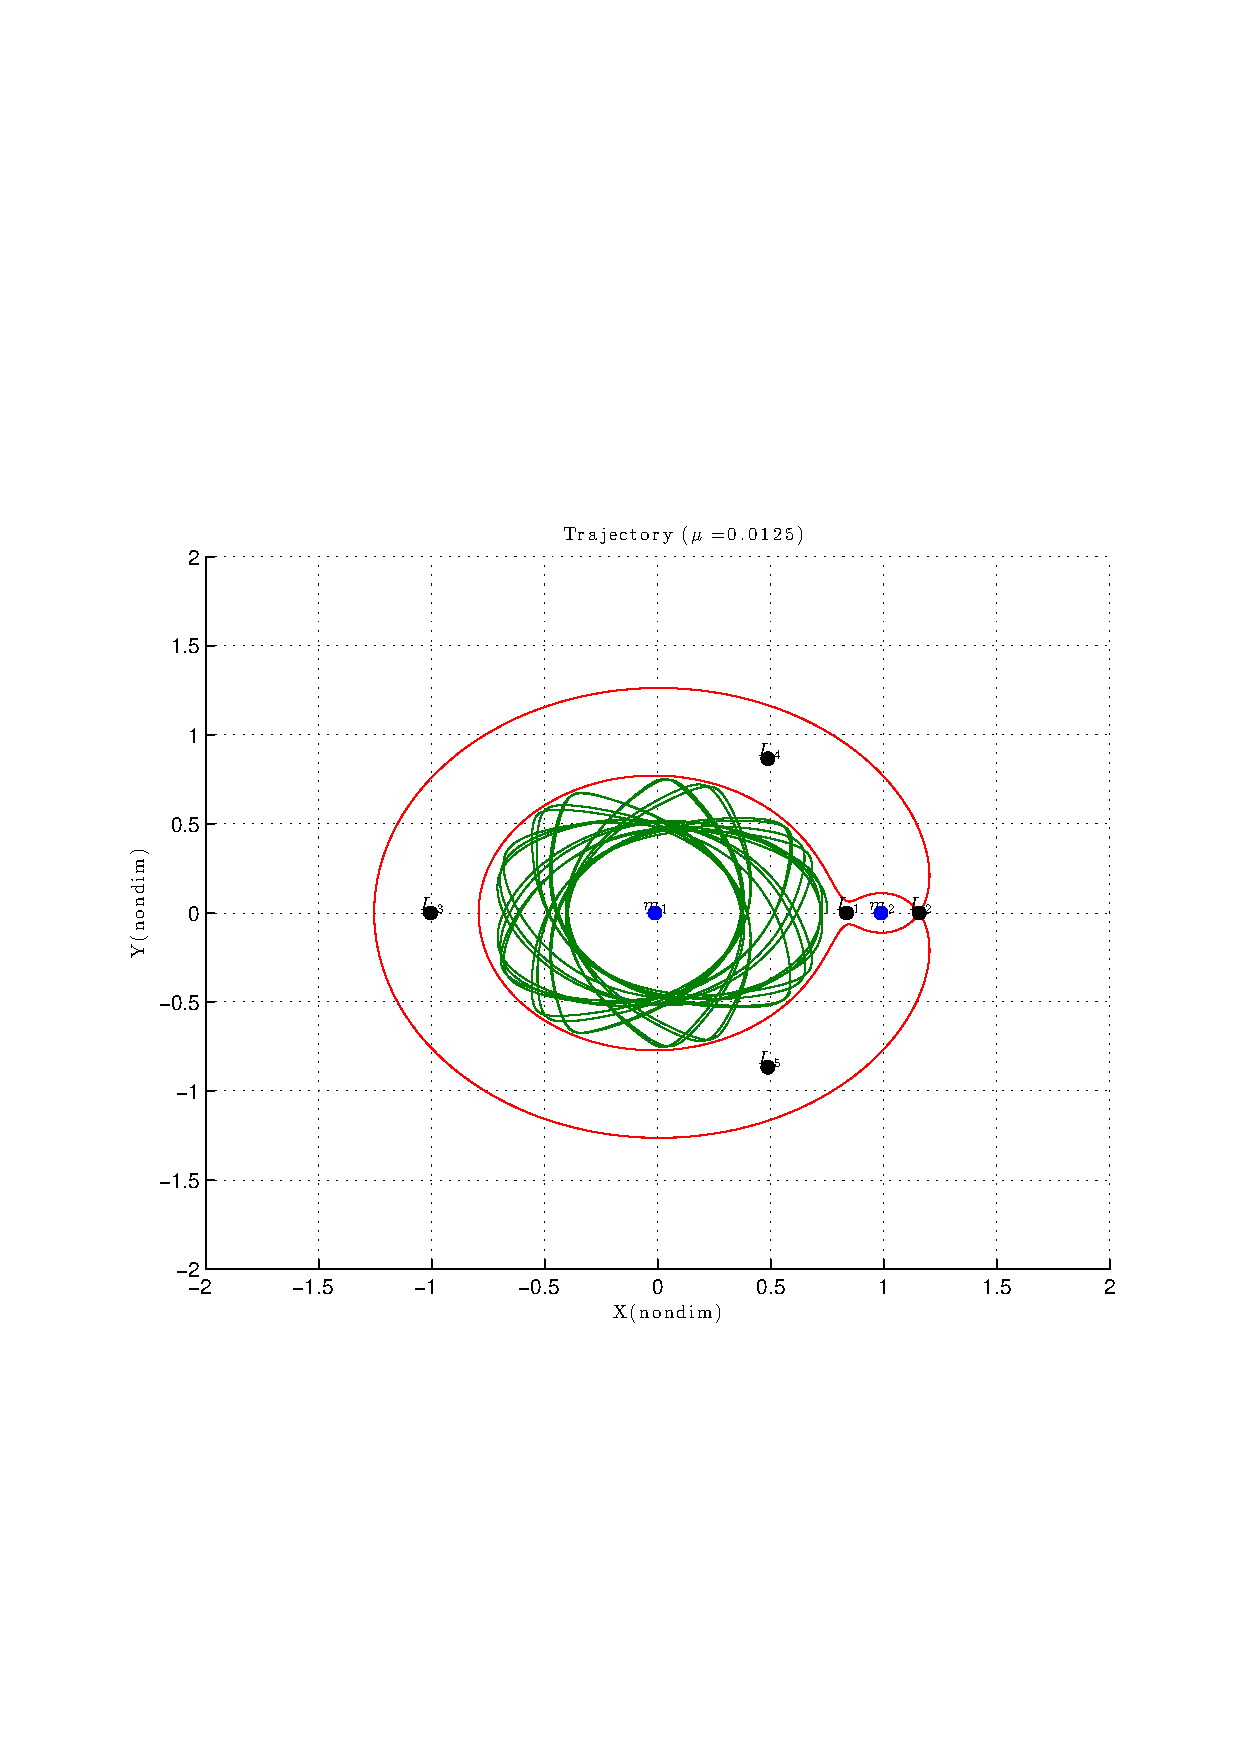
\includegraphics[width=\textwidth]{./integrator_compare/trajectory} 
		\caption{Trajectory} \label{fig:compare_trajectory} 
	\end{subfigure}~ %add desired spacing between images, e. g. ~, \quad, \qquad, \hfill etc. %(or a blank line to force the subfigure onto a new line) 
	\begin{subfigure}[htbp]{0.4\textwidth} 
		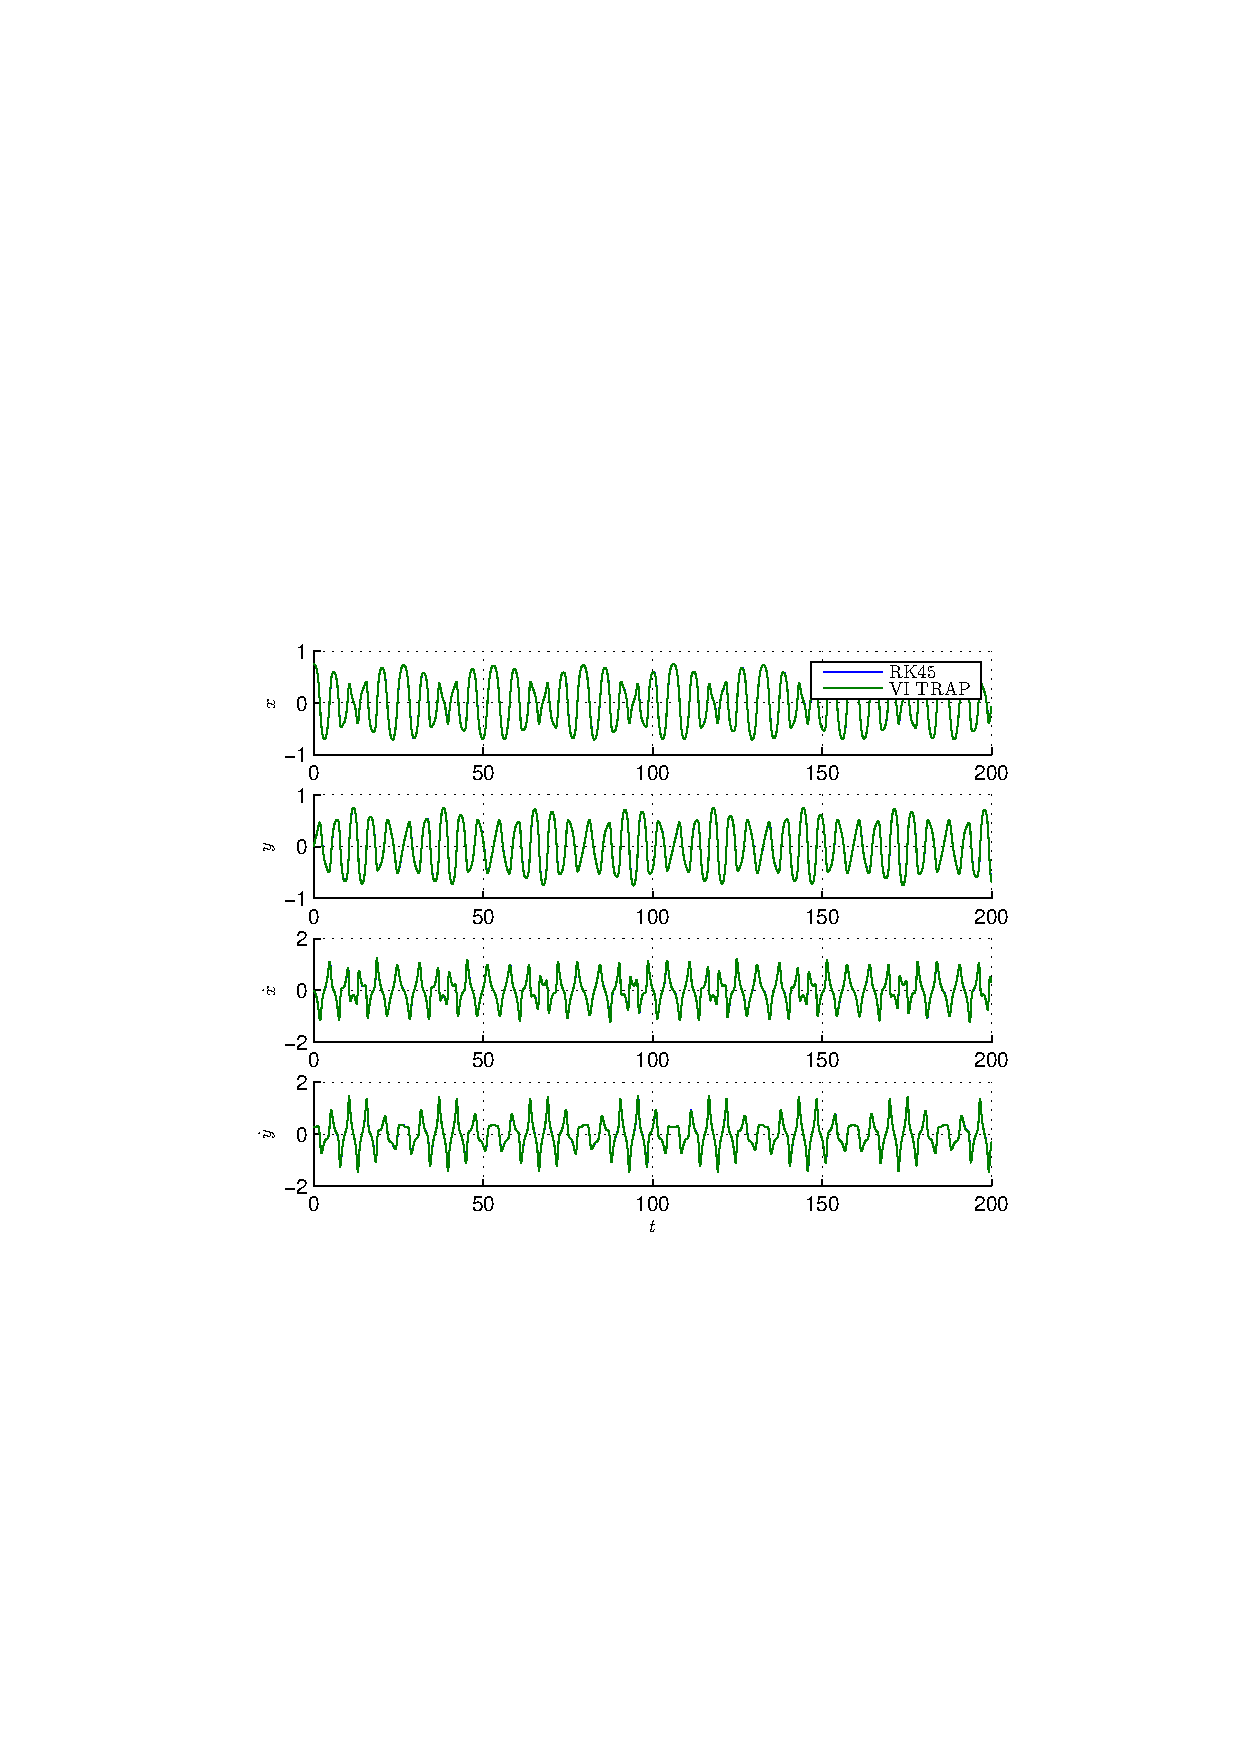
\includegraphics[width=\textwidth]{./integrator_compare/components} 
		\caption{Components} \label{fig:compare_components} 
	\end{subfigure} ~ %add desired spacing between images, e. g. ~, \quad, \qquad, \hfill etc. %(or a blank line to force the subfigure onto a new line) 
	\begin{subfigure}[htbp]{0.4\textwidth} 
		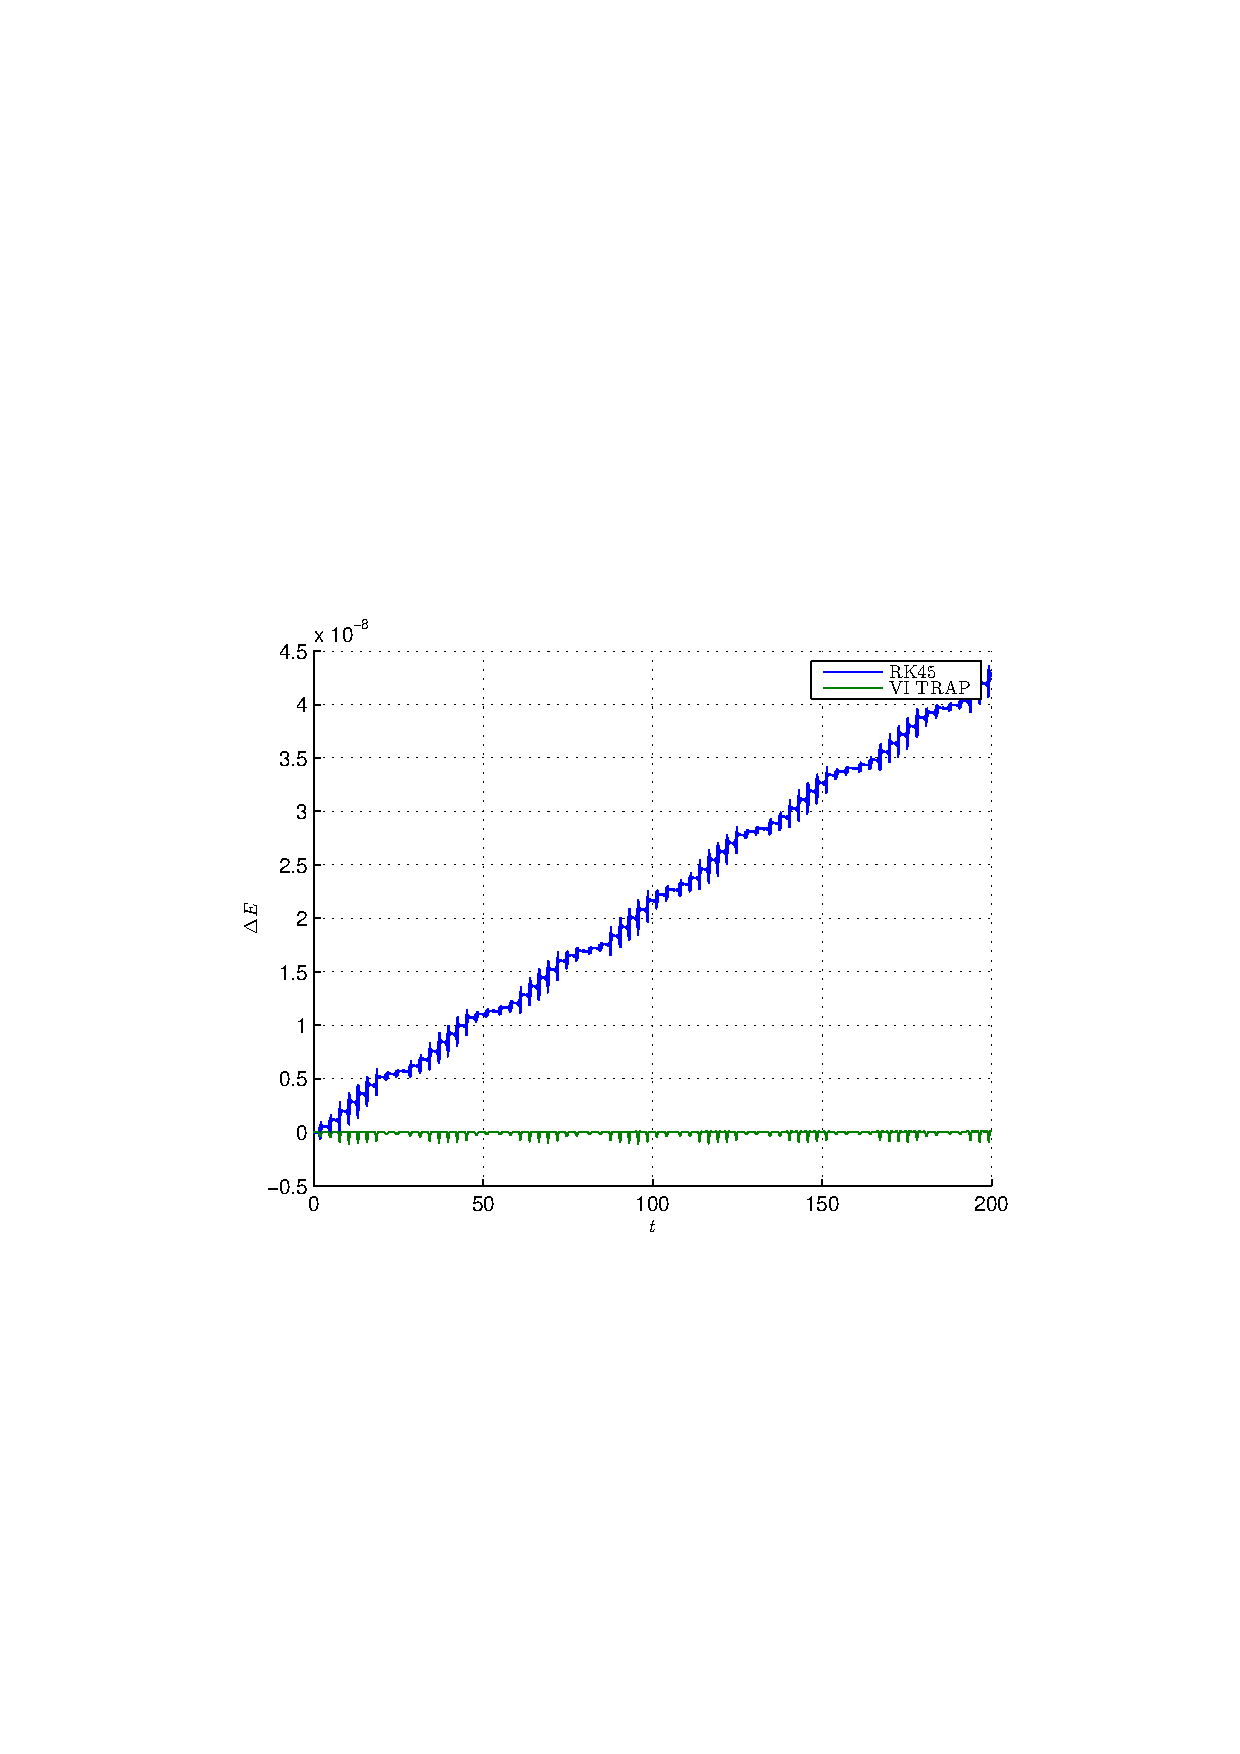
\includegraphics[width=\textwidth]{./integrator_compare/energy} 
		\caption{Energy} \label{fig:compare_energy} 
	\end{subfigure} 
	\caption{Integrator Comparison}
	\label{fig:integrator_compare} 
\end{figure}

\section{Optimal Control Formulation}\label{sec:optimal_control}
Optimal control theory has been widely applied to spacecraft trajectory design problems~\cite{peng2014,yue2009}.
Indirect optimal control allows for the calculation of state and control histories that minimize a cost functional. 
The concept of reachable sets has also seen widespread interest in the optimal control and system verifications communities. 
Given an initial condition and fixed horizon, the reachable set is the set of states attainable subject to the control constraints, which is closely related to optimal control theory~\cite{lygeros2004,lygeros2002,mitchell2002}.
In addition, the concept of reachability has also been more recently applied to the space domain~\cite{holzinger2012,holzinger2011,komendera2012a}. 
In this work, we seek to combine the concepts of reachable states with that of the Poincar\'e section in order to design orbital transfers.

The cost function is defined as
\begin{equation}
	J = -\frac{1}{2} \left( \bar{x}(t_f) - \bar{x}_{n}(t_f)\right)^T 
	\left[
	\begin{array}{cccc}
		1 & 0& 0& 0 \\
		 0& 0& 0& 0\\
		 0 & 0 & 1 &0\\
		 0 & 0& 0& 0
	\end{array}
	\right]
	\left( \bar{x}(t_f) - \bar{x}_{n}(t_f)\right)
	\label{eq:cost}
\end{equation}
The term \( \bar{x}_n(t_f) \) is the final state of a control free trajectory while the term \( \bar{x}(t_f) \) is the final state under the influence of the control input.
In this fashion, the aim is to maximize the distance of the final state from that of no control trajectory. 
A chosen Poincar\'e section is defined through the use of appropriate terminal constraints
\begin{subequations}
\begin{align}
     m_1 &= 0 = \frac{y(t_f) - L_{1y}}{x(t_f) - L_{1x}} - \tan{\alpha_d} \\ 
    m_2&= 0 = \frac{\dot{x}(t_f) - \dot{x_n}(t_f) }{x(t_f) -x_n(t_f) } - \tan{\theta_d} \\
    m_3 &= \begin{cases}
    	-\dot{x}(t_f) &\leq 0 \quad \text{if } 0 \leq \theta_d \leq \pi \\
		\dot{x}(t_f) &\leq 0 \quad \text{if } \pi \leq \theta_d \leq 2 \pi
    \end{cases}  \\
	 0 &\geq\bar{u}^T \bar{u} - u_{max}^2 
\end{align}
    \label{eq:constraints}
\end{subequations}
where the angles \( \alpha_d\) and \( \theta_d\) define the Poincar\'e section and a specific direction upon the section, respectively. 
The goal is to determine the control input \( \bar{u}(t)\) such that the cost function~\eqref{eq:cost} is minimized subject to the state equations of motion~\eqref{eq:cont_eom} and constraints~\eqref{eq:constraints}.
Application of the Euler-Lagrange equations allows us to derive the necessary conditions for optimality~\cite{bryson1975}.
\begin{subequations}\label{eq:necc_cond}
\begin{align}
	\dot{\lambda}^T &= - \frac{\partial H}{\partial x} \\
	0 &=  \frac{\partial H}{\partial u} \\
	0 &= \left[\frac{\partial \phi}{\partial x} + \beta^T \frac{\partial m}{\partial x} - \lambda^T(t_f) \right]^T \delta x(t_f) + \left. \left[ H^* + \frac{\partial \phi}{\partial t} \right] \right|_{t_f} \delta t
\end{align}
\end{subequations}
where the Hamiltonian \(H\) is defined as
\begin{equation}
	H = \lambda_r^T \bar{v} + \lambda_v^T \begin{bmatrix}0 & 2\\-2 & 0 \end{bmatrix} \bar{v} + \lambda_v^T \begin{bmatrix} U_x \\ U_y \end{bmatrix} + \lambda_v^T \bar{u}
	\label{eq:hamiltonian_opt}
\end{equation}
and \(\lambda \in \R^{n \times 1}\) is the costate and \(\beta \in \R^{3 \times 1} \) are the additional Lagrange multipliers associated with the terminal constraints in~\eqref{eq:constraints}.
This indirect optimal control formulation leads to a two point boundary value problem with split boundary conditions. 
By sweeping the angle \( \theta_d \) one can approximate the reachable set on the Poincar\'e section subject to the bounded control input. 

A numerical test case is presented to demonstrate this process and generate preliminary results.
The goal is to determine a transfer trajectory between two planar periodic orbits of the Earth-Moon system. 
The initial and target orbits are depicted in Figure~\ref{fig:opt_reach_trajectory} as the black periodic orbits.
From the initial state, a series of optimal trajectories are generated which all intersect the desired Poincar\'e section.
The intersection of these trajectories with the Poincar\'e section is shown in Figure~\ref{fig:north_poincare_reach}.
The reachable set is discretely approximated as the area enclosed by the optimal trajectories.
As the target state does not lie within the reachable set, another iteration of the optimal control calculation must be performed. 
The location on the reachable surface which lies closest to the target state is used to generate the initial conditions for the next iteration.
A second, or southern, trajectory calculation once again generates an approximation of the reachable set as shown in Figure~\ref{fig:south_reach}.
In this iteration, that target state is enclosed within the reachable set. 
\Cref{fig:opt_reach_trajectory} illustrates the completed optimal transfer trajectory.
As the solution is composed of two distinct optimal solutions there exists a discontinuity at the switching point.
This discontinuity is most evident in the control history shown in \Cref{fig:opt_reach_control}.
More general transfers would require multiple applications of this reachability computation and additional Poincar\'e sections.
This recursive method allows one to enlarge the attainable states on the Poincar\'e section.
General transfers are possible by combining powered segments along the invariant manifolds.

Cost function

Maximize a distance on the Poincar\`e section

Necessary conditions for optimality

Discrete version of costate equations of motion

Avoid explicit inverse by using gauss jordan elimination

Plot to compare continuous and discrete costate equations of motion

\section{Numerical Example}\label{sec:simulation}
Transfer between a periodic orbit and the Moon

Multiple Shooting method (choose interior patch points to decrease sensitivity)

Determine reachable set on Poincar\`e Section

Intersection of the sets on section

Minimization to a target state

Show transfer to the moon

Compare with the Ross work and the invariant manifold ( long time of flight)
\section{Conclusion}\label{sec:conclusion}

Summary of work

concrete sentence of contribution and areas of future study

\bibliographystyle{AAS_publication}   % Number the references.
%\bibliography{references}   % Use references.bib to resolve the labels.
\bibliography{library}



\end{document}
